\subsubsection{Understanding the AST}
\label{sec:AST}

The \ast{} of a typical \lang{} program can typically be divided into three
sections; the program layer, the function layer and the expression layer (see
figure~\ref{fig:astStruct}). Each node in the \ast{} correspond one-to-one with a
type of expression in \lang{} but without loss of generality they will just be
refered to as nodes or expressions.

\begin{figure}[ht]
  \centering
  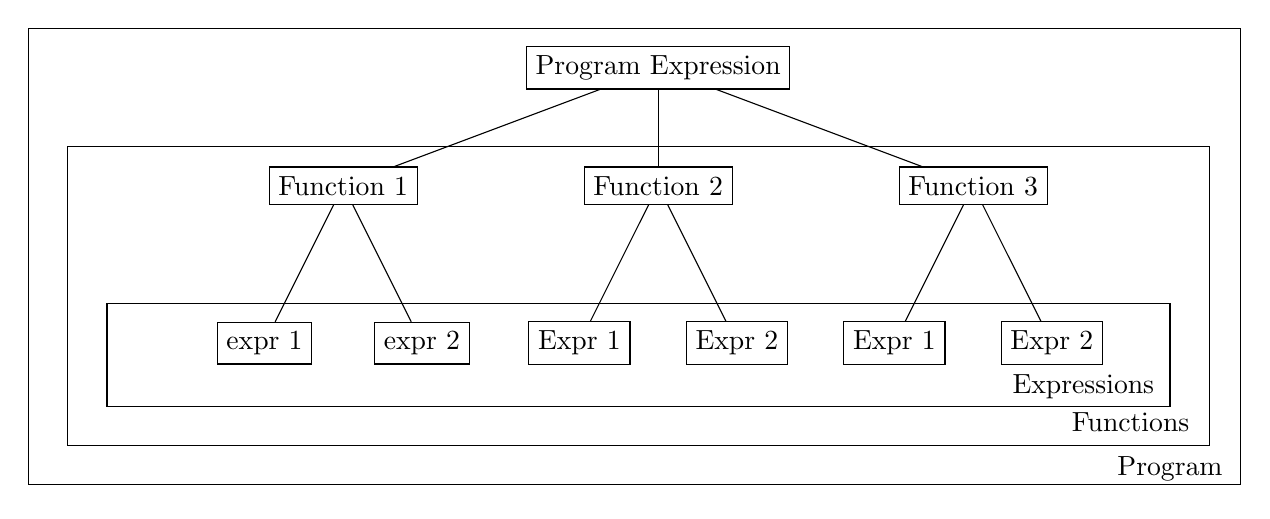
\begin{tikzpicture}
    \node[draw] (program) at (0, -0.5) {Program Expression};

    \def\functions{{Function 1}, {Function 2}, {Function 3}};
    \def\instructions{{Expr 1}, {Expr 2}}

    \foreach \fun [count=\i] in \functions {

      \pgfmathtruncatemacro{\x}{(-8 + (\i)*4)};
      \node[draw] (func\i) at (\x, -2) {\fun};
      \draw[] (program) -- (func\i); 

      
    }

    \node[draw] (int1) at (-5,-4) {expr 1};
    \node[draw] (int2) at (-3,-4) {expr 2};

    \draw[] (func1) -- (int1);
    \draw[] (func1) -- (int2);
    
    \node[draw] (int3) at (-1,-4) {Expr 1};
    \node[draw] (int4) at (1,-4) {Expr 2};

    \draw[] (func2) -- (int3);
    \draw[] (func2) -- (int4);
    
    \node[draw] (int5) at (3,-4) {Expr 1};
    \node[draw] (int6) at (5,-4) {Expr 2};

    \draw[] (func3) -- (int5);
    \draw[] (func3) -- (int6);
 
    \draw[] (-8,0) rectangle (7.4,-5.8);
    \draw[] (-7.5,-1.5) rectangle (7,-5.3);
    \draw[] (-7,-3.5) rectangle (6.5,-4.8);

    \node[] (programBox) at (6.5, -5.6) {Program};
    \node[] (functionBox) at (6, -5) {Functions};
    \node[] (instructionBox) at (5.4, -4.55) {Expressions};
  \end{tikzpicture}
  \caption{\ast{} for \lang{} showing how a typical program is structured after
  being parsed by the \lang{} parser. Each expression node, can then be further
subdivided until reaching the leafs of each branch which corresponds to terminal
expressions.}
  \label{fig:astStruct}
\end{figure}

It is this structure on which the \typeChecker, the \borrowChecker, and the
\codeGen{} will operate to produce an object file which the \gcc{} can turn into an
excutable file. The use of the visitor pattern (see section~\ref{sec:VisitorDesign}) is
specifically used to facilitate a depth first left to right traversal of the \ast{} to do
type checking, borrow checking and code generation.

This ensures the code is analyzed in the same order in which it appears in the
source code.
